\begin{figure}[bth]
    \centering
    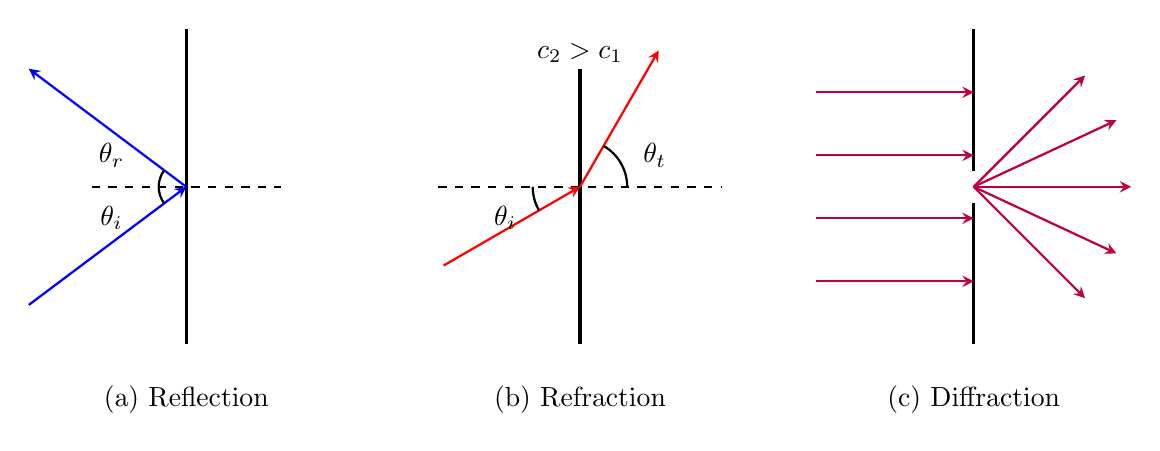
\begin{tikzpicture}[scale=1.0, thick, >=stealth]

    %========================
    % Panel (a): Reflection
    %========================
    \begin{scope}[shift={(0,0)}]
        % Boundary
        \draw[very thick] (0,0) -- (0,4);
        %\node[rotate=90] at (-0.45,2) {Boundary};

        % Normal
        \draw[dashed] (-1.2,2.0) -- (1.2,2.0);
        %\node at (1.35,2.5) {Normal};

        % Incident wave
        \draw[->, blue] (-2,0.5) -- (0,2.0);
        %\node[blue] at (-1.6,1.2) {Incident};

        % Reflected wave
        \draw[->, blue] (0,2.0) -- (-2,3.5);
        %\node[blue] at (-1.6,3.7) {Reflected};

        % Angles
        \draw (-0.35,2.0) arc[start angle=180,end angle=217,radius=0.35];
        \node at (-0.95,1.6) {$\theta_i$};

        \draw (-0.35,2.0) arc[start angle=180,end angle=143,radius=0.35];
        \node at (-0.95,2.4) {$\theta_r$};

        % Label
        \node at (0,-0.7) {(a) Reflection};
    \end{scope}

    %========================
    % Panel (b): Refraction (explicit angles)
    %========================
    \begin{scope}[shift={(5,0)}]

        % Interface (vertical)
        \draw[very thick] (0,0) -- (0,3.5);

        % Normal (horizontal, pointing to the right)
        \draw[dashed] (-1.8,2) -- (1.8,2);
        %\node at (2.0,2) {Normal};

        % Incident ray: -30° from normal
        % Direction = 180 - 30 = 150 degrees
        \draw[<-, red] (0,2) -- ++(210:2);
        %\node[red] at (-1.7,2.7) {Incident};

        % Transmitted ray: +60° from normal
        % Direction = 0 + 60 = 60 degrees
        \draw[->, red] (0,2) -- ++(60:2);
        %\node[red] at (1.6,3.2) {Refracted};

        % Incident angle theta_i (between normal and incident ray)
        \draw (-0.6,2)
            arc[start angle=180,end angle=210,radius=0.6];
        \node at (-0.95,1.6) {$\theta_i$};

        % Transmitted angle theta_t (between normal and refracted ray)
        \draw (0.6,2)
            arc[start angle=0,end angle=60,radius=0.6];
        \node at (0.95,2.4) {$\theta_t$};

        % velocity labels
        \node at (0,3.7) {$c_2 > c_1$};

        % Panel label
        \node at (0,-0.7) {(b) Refraction};

    \end{scope}

    %========================
    % Panel (c): Diffraction
    %========================
    \begin{scope}[shift={(10,0)}]
        % Barrier with aperture
        \draw[very thick] (0,0) -- (0,1.8);
        \draw[very thick] (0,2.2) -- (0,4);
        %\node[rotate=90] at (-0.45,2) {Barrier};

        % Incident waves
        \foreach \y in {0.8,1.6,2.4,3.2} {
            \draw[->, purple] (-2,\y) -- (0,\y);
        }
        %\node[purple] at (-1.6,0.5) {Incident};

        % Diffracted waves
        \foreach \angle in {-45,-25,0,25,45} {
            \draw[->, purple] (0,2) -- ++(\angle:2);
        }
        %\node[purple] at (1.7,3.5) {Diffracted};

        % Label
        \node at (0,-0.7) {(c) Diffraction};
    \end{scope}

    \end{tikzpicture}
    \caption{Schematic illustration of (a) reflection, (b) refraction, and (c) diffraction of waves.  Dashed lines indicate the surface normal relevant to Snell's law.  Geometry is schematic and not to scale.}
    \label{fig:wave_phenomena}
\end{figure}